\documentclass[oneside, final, 14pt]{article}
\usepackage[utf8]{inputenc}
\usepackage[russianb]{babel}
\usepackage{vmargin}
\setpapersize{A4}
\setmarginsrb{2cm}{1.5cm}{1cm}{1.5cm}{0pt}{0mm}{0pt}{13mm}
\usepackage{indentfirst}
\usepackage{graphicx}
\usepackage{amsmath}
\usepackage{amssymb}
\usepackage{amsthm}
\usepackage {titlesec}
\usepackage{algorithm}
\usepackage{algpseudocode}
\bibliographystyle{unsrt} 
%\usepackage{biblatex}
\begin{document}
\sloppy
	\renewcommand\contentsname{Содержание} %%% renaming the Table of Contents
%	\renewcommand\chaptername{}
%	\renewcommand\chapternum{}
%	\thispagestyle{empty}

\begin{titlepage}
\begin{center}
\bfseries
Московский Государственный Университет \\имени М.~В.~Ломоносова\\
Факультет вычислительной математики и кибернетики\\
Кафедра математической физики\\

\includegraphics[width=0.4\textwidth]{msu_logo_small.png}\\
\vfill	

\mdseries
\begin{Large}
КУРСОВАЯ РАБОТА СТУДЕНТА 402 ГРУППЫ\\
\end{Large}
Турганбаева Сатбека Амангельдыулы\\
\vfill	
Тема курсовой работы:\\
\vspace{1cm}
\bfseries
\begin{Large}
"О тестах для схем при некоторых \\	замещающих неисправностях"\\
\end{Large}
\vfill	

  \begin{flushright}
        Научный руководитель:\\
        д.ф-м.н. профессор Разгулин~А.~В.
    \end{flushright}

\vfill	


\end{center}

\begin{center}
	Москва 2017
\end{center}

\end{titlepage}

\tableofcontents

\newpage
\section*{Введение}
\addcontentsline{toc}{section}{Введение}
Системы адаптивной оптики используемые в современных телескопах используют гибкие зеркала, для коррекции аберраций, вызванных турбулентность атмосферы Земли. Одним из устройств для измерения волнового фронта является датчик Шака-Гартмана. Данный датчик измеряет градиент волнового фронта, вместо него самого. Получаются матрицы градиентов $X$ и $Y$.

Метод, рассматриваемый в данной работе заключается в получении из матриц градиента $X$, $Y$ стандартного разложения по вейвлетам Хаара исходного волнового фронта, и применении к полученному результату стандартного алгоритма синтеза. В результате восстанавливается исходный волновой фронт.


\section{Преобразование Хаара.}
\subsection{Формулировки и определения}
\textbf{Z-преобразованием} дискретного сигнала $\{s_j\}_{ j \in Z}$ называется полином Лорана 
$P_{s}(z) = \sum_{j \in Z} s_{j}z^{-j}$.

$h = (\frac{1}{\sqrt{2}}, \frac{1}{\sqrt{2}}),~g = (\frac{1}{\sqrt{2}}, -\frac{1}{\sqrt{2}})$ - низкочастотный и высокочастотный фильтры преобразования Хаара.

$$ H_{L}(z) = \frac{1 + z^{-1}}{\sqrt{2}} $$
$$ H_{H}(z) = \frac{1 - z^{-1}}{\sqrt{2}} $$
$H_{L}(z)$,~$H_{H}(z)$ - z - преобразования фильтров $h$ и $g$ соответственно.

\textbf{Линейной сверткой} двух дискретных сигналов $a(n),~ n=0 \ldots N-1$ и $b(n),~ n=0 \ldots M-1$ называется выражение:
$$ h = a \otimes b $$
$$ h(n) =  \sum_{m=0}^{n} a(m)b(n-m) $$
В ввиду того, что сигналы конечномерные на границах возникает неопределенность из-за отсутствия соответствующих элементов. Проблема решается различными способами: дополнение одного из обоих сигналов $0$-ми, константами, симметричное отражение и т.д.

Также одним из свойств $z$-преобразования является то, что $z$-преобразование свертки двух сигналов равно произведению $z$-преобразований этих сигналов. 

\textbf{$\uparrow s$} - операция, добавляющая $0$ после каждого элемента сигнала $s$.

\textbf{$\downarrow_k s$} - операция, удаляющая каждый $k$-ый элемент сигнала $s$.

Если $s = (1,2,3,4)$, то $\uparrow_2 s = (1,0,2,0,3,0,4,0)$, а $\downarrow_{2} s = (1,3)$.

Также стоит отметить, что:
$$\downarrow_2 H_L(z^{2^k}) = H_L(z^{2^{k-1}}),~ k\geq 2$$
$$\downarrow_2 H_H(z^{2^k}) = H_H(z^{2^{k-1}}),~ k\geq 2$$
$$\uparrow_2 H_L(z^{2^{k-1}}) = H_L(z^{2^{k}}),~ k\geq 2$$
$$\uparrow_2 H_H(z^{2^{k-1}}) = H_H(z^{2^{k}}),~ k\geq 2$$

В дальнейшем под сигналом будет пониматься его $z$-преобразование и наоборот.
\subsection{Одномерный сигнал}
Будем предполагать в дальнейшем, что размерность сигналов равна $2^m,~m \geq~1$.

Свернем сигнал $h_m(z)$, $dim~h_m = 2^m$ с фильтрами $H_L(z)$,~$H_H(z)$, а затем применим к получившемуся операцию $\downarrow_2$.

Получим сигналы: $$h_{L_{m-1}}(z) = \downarrow_2 \{h_m(z)H_L(z)\}$$ $$h_{H_{m-1}}(z) = \downarrow_2 \{h_m(z)H_H(z)\}.$$ Их размерности будут в два раза меньше,размерности исходного сигнала $h_m$.

$h_{L_{m-1}}(z)$ называется низкочастотной составляющей сигнала $h_m$, a $h_{H_{m-1}}(z)$ высокочастотной. 

Восстановление исходного сигнала происходит так:
$$h_m(z) = \uparrow_2 \{ h_{L_{m-1}}(z) \} H_L(z) + \uparrow_2 \{ h_{H_{m-1}}(z) \} H_H(z)	$$
Описанные выше преобразования выполняют один шаг прямого и обратного преобразования Хаара. Прямое преобразование называется анализом, обратное синтезом.

Если положить, что $h_m = h_{L_m}$, то алгоритм анализа выглядит так:
\begin{algorithm}
\caption{Алгоритм анализа}
\begin{algorithmic}
	\For{$k=1 \ldots m$}
	\State $h_{L_{m-k}}(z) = \downarrow_2 \{h_{L_{m-k+1}}(z)H_L(z)\}$
	\State $h_{H_{m-k}}(z) = \downarrow_2 \{h_{L_{m-k+1}}(z)H_H(z)\}.$
	\EndFor
\end{algorithmic}
\end{algorithm}


$k$ называется разрешением разложения. Анализ будет происходить до тех пор, пока не останется один элемент.
\begin{algorithm}[H]
\caption{Алгоритм синтеза}
\begin{algorithmic}
	\For{$k=m \ldots 1$}
		\State$h_{L_{m-k + 1}}(z) = \uparrow_2 \{ h_{L_{m-k}}(z) \} H_L(z^{-1}) + \uparrow_2 \{ h_{H_{m-k}}(z) \} H_H(z^{-1})$
	\EndFor
\end{algorithmic}
\end{algorithm}	

\subsection{Дополнение нулями}
В описываемом методе при анализе будем дополнять нулями справа, а при синтезе слева. Ниже приведены примеры анализа и синтеза сигнала $(1,2,3,4)$. Для наглядности используется нестандартные пары фильтров, $[1,1]$, $[1,-1]$ и $[0.5,0.5]$, $[0.5,-0.5]$.
\begin{center}
\center{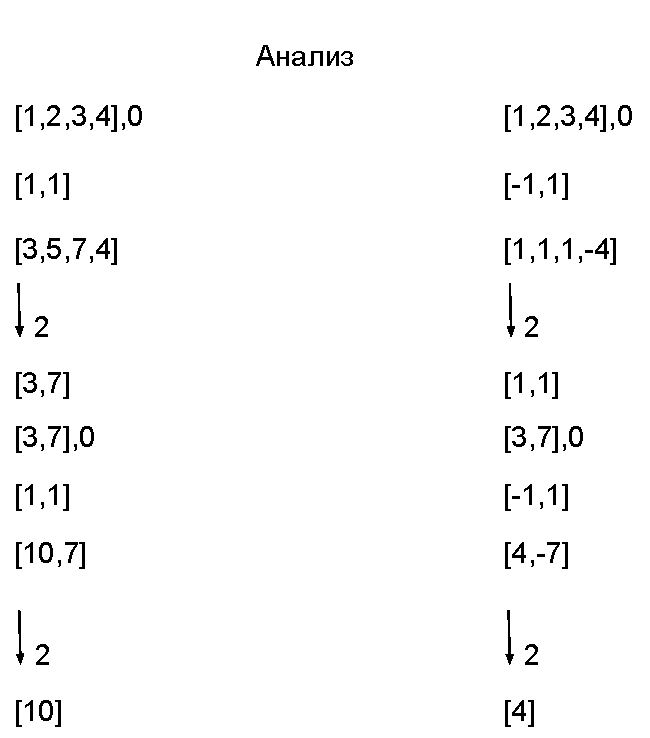
\includegraphics[width=0.6\linewidth]{analyze.pdf}}
\center{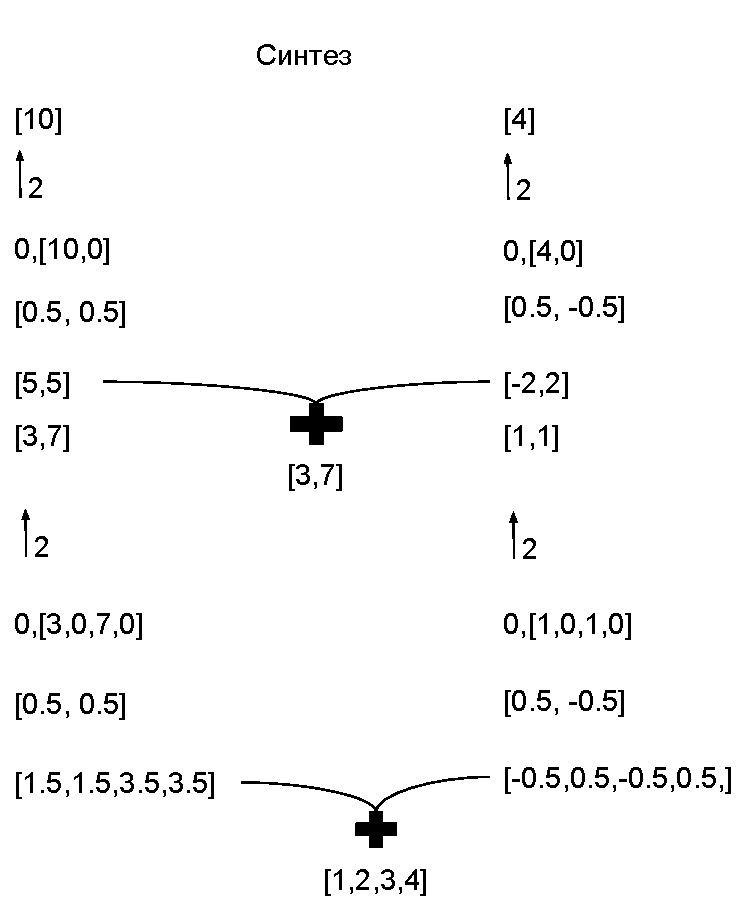
\includegraphics[width=0.6\linewidth]{synthesis.pdf}}
\end{center}


\subsection{Двумерное преобразование}
Пусть дана матрица $^{M}\Phi, ^{M}\Phi \in \mathbb{R}^{2^{M}\times2^{M}}$. Применим к каждой строке матрицы один шаг анализа. В результате получим матрицы $_L^{m-1}\Phi$, $_H^{m-1}\Phi$. К каждому столбцу обеих матриц также применим шаг анализа. В итоге получим четыре матрицы $_{LL}^{m-1}\Phi$, $_{LH}^{m-1}\Phi$, $_{HL}^{m-1}\Phi$, $_{HH}^{m-1}\Phi$. $_{LL}^{m-1}\Phi$ - является низкочастотной составляющей двумерного сигнала, остальные три матрицы содержат детализирующую информацию. Таким образом будет выполнен первый шаг двумерного преобразования Хаара. Нужно проделать аналогичные операции с $_{LL}^{m-1}\Phi$ для следующего шага. Такми образом, шаг двумерного преобразования свелся к композиции одномерных преобразований.

Синтез происходит аналогичным образом: в обратном анализу порядке дополняется нулями соответствующая размерность и применяются фильтры Хаара, а затем результаты складываются.

Пусть $^{M}\Phi = _{LL}^{M}\Phi$
\begin{algorithm}[H]
\caption{Алгоритм 2D-анализа}
\begin{algorithmic}
	\For{$k=M \ldots 1$}
		\State $_{LL}^{k-1}\Phi = \downarrow_{2}$ $\{_{LL}^{k}\Phi H_{L}(z_h)H_{L}(z_v)\}$
		\State $_{LH}^{k-1}\Phi = \downarrow_{2}$ $\{_{LL}^{k}\Phi H_{L}(z_h)H_{H}(z_v)\}$
		\State $_{HL}^{k-1}\Phi = \downarrow_{2}$ $\{_{LL}^{k}\Phi H_{H}(z_h)H_{L}(z_v)\}$
		\State $_{HH}^{k-1}\Phi = \downarrow_{2}$ $\{_{LL}^{k}\Phi H_{H}(z_h)H_{H}(z_v)\}$
	\EndFor
\end{algorithmic}
\end{algorithm}
\begin{algorithm}[H]
\caption{Алгоритм 2D-синтеза}
\begin{algorithmic}
	\For{$k=1 \ldots M$}
	\State  $_{LL}^{k-1}\Phi=$ $\uparrow_2$  $\{_{LL}^{k-1}\Phi H_L(z_v^{-1}) + _{LH}^{k-1}\Phi H_L(z_v^{-1})\}H_L(z_h^{-1})+ $ $\uparrow_2$ $\{_{HL}^{k-1}\Phi H_L(z_v^{-1}) + _{HH}^{k-1}\Phi H_L(z_v^{-1})\}H_H(z_h^{-1})$
	\EndFor
\end{algorithmic}
\end{algorithm}	
Полученное $2$-$D$ разложение можно представить в виде диаграммы, где на каждом уровне $LL$, $LH$, $HL$ и $HH$ составляющим соответствуют определенные квадранты. 
\begin{center}
\center{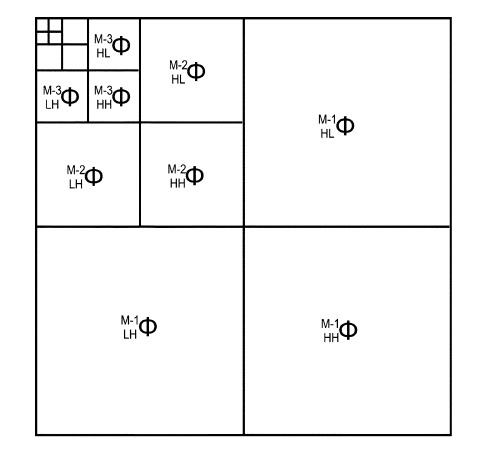
\includegraphics[width=0.6\linewidth]{hwaf_decomp.png}}
\end{center}
\subsection{Явные формулы для анализа}
Из алгоритма анализа непосредственно выводятся формулы для $LL$, $LH$, $HL$ и $HH$ составляющих на каждом уровне.
\begin{equation}\label{LL}
_{LL}^{M-m}\Phi=
\downarrow_{2^m} \{^M\Phi\prod\limits_{k = 0}^{m-1} H_L(z_h^{2^k})
							\prod\limits_{k = 0}^{m-1} H_L(z_v^{2^k})\}
\end{equation}
\begin{equation}\label{LH}
_{LH}^{M-m}\Phi=
\downarrow_{2^m} \{^M\Phi H_H(z_v^{2^{m-1}}) \prod\limits_{k = 0}^{m-1} H_L(z_h^{2^k})
							\prod\limits_{k = 0}^{m-2} H_L(z_v^{2^k})\}
\end{equation}
\begin{equation}\label{HL}
_{HL}^{M-m}\Phi=\downarrow_{2^m} \{^M\Phi H_H(z_h^{2^{m-1}}) \prod\limits_{k = 0}^{m-2} H_L(z_h^{2^k})
						\prod\limits_{k = 0}^{m-1} H_L(z_v^{2^k})\}
\end{equation}
\begin{equation}\label{HH}
_{HH}^{M-m}\Phi=\downarrow_{2^m} \{^M\Phi H_H(z_v^{2^{m-1}}) H_H(z_v^{2^{m-1}}) \prod\limits_{k = 0}^{m-2} H_L(z_h^{2^k})
							\prod\limits_{k = 0}^{m-2} H_L(z_v^{2^k})\}
\end{equation}
\section{Градиенты. Геометрия Хаджина и Фрайда.}
\subsection{Геометрия Хаджина и Фрайда}
В адаптивной оптике используются два различных способа представления наклонов волнового фронта. Согласно \cite{how}
это геометрии Хаджина и Фрайда.
Геометрия Хаджина:
$$_{H}x_{i,j}=-\phi_{i,j}+\phi_{i,j+1}$$
$$_{H}y_{i,j}=-\phi_{i,j}+\phi_{i+1,j}$$
Получившиеся матрицы $_H^{M}X$, $_H^{M}Y$ имеют размерности $2^M \times(2^M - 1)$ и $(2^M - 1) \times 2^M$ соответственно.
Геометрия Фрайда:
$$_{F}x_{i,j}=\frac{_{H}x_{i,j} + _{H}x_{i+1,j}}{2} = \frac{-\phi_{i,j}+\phi_{i,j+1}-\phi_{i+1,j}+\phi_{i+1,j+1}}{2}$$
$$_{F}y_{i,j}=\frac{_{H}y_{i,j} + _{H}y_{i,j+1}}{2} = \frac{-\phi_{i,j}-\phi_{i,j+1}+\phi_{i+1,j}+\phi_{i+1,j+1}}{2}$$
Получившиеся матрицы $_F^{M}X$, $_F^{M}Y$ имеют одинаковые размерности $2^M - 1 \times 2^M - 1$.
\subsection{Градиенты и преобразование Хаара.}
Справедливы следующие соотношения.
\begin{equation}\label{_H^MX}
_H^MX = ^M\Phi\sqrt{2}H_H(z_h) 
\end{equation}
\begin{equation}\label{_H^MY}
_H^MY = ^M\Phi\sqrt{2}H_H(z_v)
\end{equation}
\begin{equation}\label{_F^MX}
_F^MX = \frac{_H^MX H_L(z_v)}{\sqrt{2}}=^M\Phi H_H(z_h) H_L(z_v)
\end{equation}
\begin{equation}\label{_F^MY}
_F^MY = \frac{_H^MY H_L(z_h)}{\sqrt{2}}=^M\Phi H_L(z_h) H_H(z_v)
\end{equation}
\section{Постановка и решение задачи.}
\subsection{Постановка задачи}
Рассмотрим случай, когда известны вертикальные и горизонтальные наклоны, а также интенсивность волнового фронта. Иначе говоря имеются: $_F^MX$, $_F^MY$, $_H^MX$, $_H^MY$ , $_0^{LL}\Phi$.

Необходимо получить из имеющихся данных получить $2D$-разложение волнового фронта, а затем восстановить сам волновой фронт, применив к полученному разложению стандартный алгоритм синтеза.\cite{new_method1}
Диаграмма разложения которое необходимо получить будем аналогична диаграмме стандартного разложения:
\begin{center}
\center{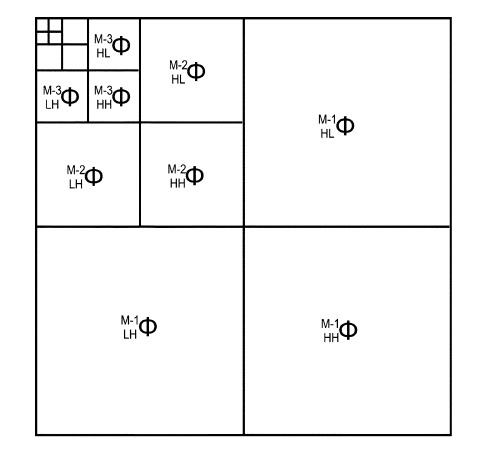
\includegraphics[width=0.6\linewidth]{hwaf_decomp.png}}
\end{center}
Отличаться будут лишь формулы (\ref{LL})-(\ref{HH}). "Идейно" метод заключается в замене переменной. Используя соотношения (\ref{_H^MX})-(\ref{_F^MY}), получим аналоги (\ref{LL})-(\ref{HH}).
\subsection{LH, HL квадранты}
Из соотношений (\ref{_H^MX}), (\ref{_H^MY}) и (\ref{HL}), (\ref{LH}) соответственно, непосредственно вытекает, что:
\begin{center}

$ 	_{HL}^{M-1}\Phi = \downarrow_{2}$ $ _F^MX $ 

$ 	_{LH}^{M-1}\Phi = \downarrow_{2}$ $ _F^MY $

\end{center}

Докажем справедливость выражения $H_{H}(z^{2^{m-1}}) = \sqrt{2}^{m-1} H_H(z) \prod \limits_{k=0}^{m-2} H_L(z^{2^k})$
\begin{proof}
Запишем $H_{H}(z^{2^{m-1}})$ в виде полинома
$$H_{H}(z^{2^{m-1}}) = \frac{1 - z^{2^{m-1}}}{\sqrt{2}}$$
$$\frac{1 - z^{2^{m-1}}}{\sqrt{2}} = \frac{(1-z^{2^{m-2}})(1+z^{2^{m-2}})}{\sqrt{2}}=\ldots=\frac{(1-z)(1+z)(1+z^2)\ldots(1+z^{2^{m-2}})}{\sqrt{2}}$$
$$H_{H}(z^{2^{m-1}}) = \sqrt{2}^{m-1} H_H(z) \prod \limits_{k=0}^{m-2} H_L(z^{2^k})$$
\end{proof}

\textbf{LH, $m>1$:}

\[
_{LH}^{M-m}\Phi=
\downarrow_{2^m} \{^M\Phi [H_H(z_v^{2^{m-1}})] [\prod\limits_{k = 0}^{m-1} H_L(z_h^{2^k})]
							\prod\limits_{k = 0}^{m-2} H_L(z_v^{2^k})\}=\]
							
\[
=\downarrow_{2^m} \{^M\Phi [\sqrt{2}^{m-1} H_H(z_v) \prod \limits_{k=0}^{m-2} H_L(z_v^{2^k})]
					[H_L(z_h)\prod \limits_{k=1}^{m-1} H_L(z_h^{2^k})]
					\prod\limits_{k = 0}^{m-2} H_L(z_v^{2^k})
\}			
\]
\[
=\sqrt{2}^{m-1} \downarrow_{2^m} \{^M\Phi H_L(z_h) H_H(z_v)\prod \limits_{k=1}^{m-1} H_L(z_h^{2^k})\prod \limits_{k=0}^{m-2} H_L^2(z_v^{2^k})
\]
\[
=\sqrt{2}^{m-1} \downarrow_{2^m} \{_F^MY \prod \limits_{k=1}^{m-1} H_L(z_h^{2^k})\prod \limits_{k=0}^{m-2} H_L^2(z_v^{2^k})
\]
\textbf{HL, $m>1$:}

Выводится аналогично, LH
\[_{HL}^{M-m}\Phi=
\sqrt{2}^{m-1} \downarrow_{2^m} \{_F^MY \prod \limits_{k=0}^{m-2} H_L^{2}(z_h^{2^k})\prod \limits_{k=1}^{m-1} H_L(z_v^{2^k})\}
\]

\subsection{HH квадрант}
\textbf{HH, $m=1$:}\cite{new_method2}

Докажем, что $_{HH}^{M-1}\Phi\downarrow_2 \{\frac{\sqrt{2}}{4}[_{H}^MX H_H(z_v) + _{H}^MY H_H(z_h)]\}$
%$_{HH}^{M-1}\Phi = \downarrow_2$ $ [^{M}\Phi H_H(z_h)H_H(z_v)]$
\begin{proof}
Известно, что $_{HH}^{M-1}\Phi = \downarrow_2$ $ [^{M}\Phi H_H(z_h)H_H(z_v)]$.

Распишем \begin{math} _{HH}^{M-1}\Phi = \downarrow_2 \{ \frac{\sqrt{2}}{2}\sqrt{2} ~^{M}\Phi H_H(z_h)H_H(z_v) \} \end{math}, выделив из (\ref{_F^MX}) $_H^MX$ получим:
\[
 _{HH}^{M-1}\Phi = \downarrow_2 \{\frac{\sqrt{2}}{2} ~_{H}^MX H_H(z_v)\} = \downarrow_2 \{\frac{\sqrt{2}}{4}2 ~_{H}^MX H_H(z_v)\}
\]

Разделив (\ref{_F^MX}) на (\ref{_F^MY}) получим:
\[
_{H}^MX H_H(z_v) = _{H}^MY H_H(z_h)
\]
Отсюда получим:
\[
_{HH}^{M-1}\Phi\downarrow_2 \{\frac{\sqrt{2}}{4}[_{H}^MX H_H(z_v) + _{H}^MY H_H(z_h)]
\]
\end{proof}

\textbf{HH, $m>1$:}
\[
_{HH}^{M-m}\Phi=\downarrow_{2^m} \{^M\Phi H_H(z_v^{2^{m-1}}) H_H(z_v^{2^{m-1}}) \prod\limits_{k = 0}^{m-2} H_L(z_h^{2^k})
							\prod\limits_{k = 0}^{m-2} H_L(z_v^{2^k})\}=\]
							
\[
=\downarrow_{2^m} \{^M\Phi \sqrt{2}^{m-1} H_H(z_h) \prod \limits_{k=0}^{m-2} H_L(z_h^{2^k})   
\prod \limits_{k=0}^{m-2} H_L(z_h^{2^k}) H_H(z_v^{2^{m-1}})H_L(z_v) \prod \limits _{k=1}^{m-2}H_L(z_v^{2^k})=
  \}
\]
\[
=\sqrt{2}^{m-1} \downarrow_{2^m} \{_F^MX \prod \limits_{k=0}^{m-2} H_L^2(z_h^{2^k}) H_H(z_v^{2^{m-1}}) \prod \limits_{k=1}^{m-2}H_L(z_v^{2k})    \}
\]
\section{Программная реализация.}
По формулам, выведенным для $HH$, $LH$, $HL$, $HH$ был написан модуль на языке Python 3.6. В модуле реализованы функции для анализа и синтеза. Модуль совместим со стандартной библиотекой для вейвлетов Pywawelets.

Пример работы программы на полиноме Цернике $_1^1R$.
\begin{figure}[h]
\center{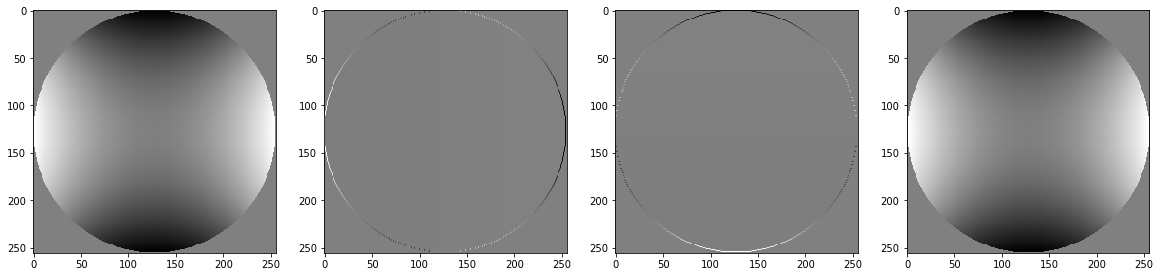
\includegraphics[width=1\linewidth]{zernike.png}}
\caption{исходное изображение, $_F^MX$, $_F^MY$, восстановленное изображение }
\end{figure}
\[MSE(x, y) = \sqrt{\frac{1}{n}\sum\limits_{i=1}^{n}(x_i - y_i)}\]
\[MSE = 3.4117657322410297e-31\]
\section{Результаты вычислительных экспериментов.}
\section{Заключение.}
Метод показал высокую точность восстановления, однако в ходе выполнения работы не было цели добиться высокой скорости его работы. В процессе написания программы стало ясно, что метод обладает ресурсом параллелизма и, что алгоритм можно оптимизировать. Также можно привести сравнение данного с другими, решающими задачу восстановления волнового фронта. Возможно также рассмотреть поведение метода при зашумленных градиентах, и некорректной интенсивности.
\bibliography{bibl}

\end{document}